
\section{Microcontrolador e IDE}

\subsection{Microcontrolador}

Microcontroladores são circuitos integrados compactos desenvolvidos para governar
uma operação específica em um sistema embarcado. No contexto da aplicação deste
trabalho, o uso de um microcontrolador é fundamental para se obter o controle
desejado de trajetória e posicionamento do robô.

Foram testadas duas placas de microcontrolador o BluePill e ESP32 Devkit v1
Ambas com processadores de 32bits
e podem ser alimentadas através dos pinos de 5v e 3.3v, mas também através do connector micro-USB-B

A escolha dessas duas placas durante o desenvolvimento foi motivada pelo custo de aquisição
e pelos componentes e opções de comunicação disponíveis.
Já se era conhecido o baixo preço da placa BluePill, e já havia sido adquirido anteriormente ao projeto.
A escolha do ESP32 Devkit v1 foi motivada também pelo custo, mas também pela
integração com bluetooth que será discutida nas seções a seguir.

A tabela \ref{precos_placas} compara a faixa de preço entre as principais placas de desenvolvimento
que podem ser encontradas para compra em território nacional.

\begin{quadro}[htb]
	\caption{Comparação de preços entre as placas de desenvolvimento \label{precos_placas}}
	 \begin{tabular}{|c|c|}
		\hline
		\textbf{Placa de desenvolvimento} & \textbf{Faixa de preço em R\$} \\ \hline
		BluePill (STM32F103C8T6) &  23 - 49 (já adquirido anteriormente) \\ \hline
		ESP32 DevKit V1  &  40 - 80   \\ \hline
		Arduino Due R3 &  320 - 470   \\ \hline
		Nodemcu v3 ESP8266 & 22 - 35   \\ \hline
		Raspberry pi pico (1, 2, W, H)  & 36 - 66  \\ \hline
	\end{tabular}
	\caption*{FONTE: Própria}
\end{quadro}

A pesquisa de preços foi feita nas principais lojas de componentes eletrônicos disponível online:
\begin{itemize}
	\item https://www.rsrobotica.com.br/
	\item https://www.robocore.net/
	\item https://www.makerhero.com/
	\item https://www.iot-robotica.com.br/
	\item https://www.ardurobotica.com.br/
	\item https://curtocircuito.com.br/
	\item https://www.saravati.com.br/
	\item https://www.a2robotics.com.br/
	\item https://www.ardurobotica.com.br/
	\item https://www.casadarobotica.com/
\end{itemize}



\subsubsection{BluePill - STM32F103C8}

A placa BluePill embarca o microcontrolador STM32F103C8.
"STM32" é uma família de microcontroladores de 32-bits fabricados pela
ST-Microelectronics. O processador empregado nessa família é o ARM Cortex-M3 \cite{cortex_m3},
baseado em arquitetura Harvard. Tem 64Kbs de memória flash.

De acordo com o \textit{livro Discovering the STM32 Microcontroller} \cite{stm_doc} e 
a documentação colaborativa do projeto STM32-base.org \cite{stm32_base_org},
possui também 7 timers, 2 ADCs, e 9 interfaces de comunicação, incluindo I2C,  USART, SPI, e USB 2.0. 
O STM32 apresenta 7 pinos que suportam canais de PWM de 5V, e outros 8 canais de 3.3V, e pode ser alimentado
via microUSB de 5V. Existem 3 grupos de pinos,  $P_{A}$,  $P_{B}$ e  $P_{C}$: os pinos PA vão de $P_{A0}$ 
a $P_{A15}$, PB indo de $P_{B0}$ a $P_{B15}$, e PC com apenas 3 pinos, $P_{C13}$, $P_{C14}$ e $P_{C15}$.
A relação geral dos pinos pode ser melhor obervada na figura \ref{stm32f103c8_pinout}.

\begin{figure}[ht]
	\centering
	\caption{Diagrama de pinos do STM32F103C8}
	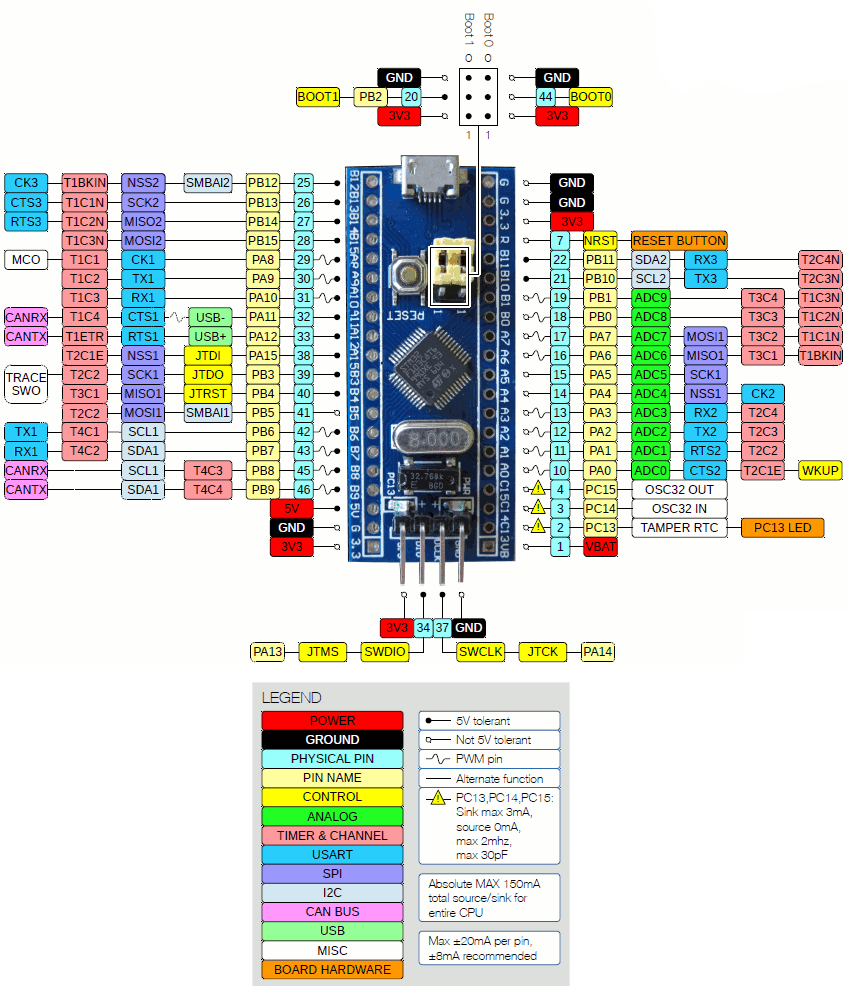
\includegraphics[width=1.0\textwidth]{figures/stm32f1_pinout}
	\caption*{FONTE: Sistemas Microprocessados -Apostila com práticas e foco nos processadores ARM CORTEX \cite{apostila_microprossados}}
    \label{stm32f103c8_pinout}
\end{figure}

Para carregar o projeto no microcontrolador, tem por padrão o uso do gravador ST-LINK v2.
O ST-link, cujo original (figura \ref{stlinkv2_original}) é fabricado pela ST-Microelectronics, 
possui uma versão paralela mais barata
comercializada online (figura \ref{stlinkv2_cheap}), porém a versão paralelo costuma ter fabricantes diversos e 
muitas vezes não descritos na distribuição do produto 
e a relação de pinos pode variar (figura \ref{stlinkv2_cheap_pin_diff}).

É possível modificar o firmware do STM32F103C8 para permitir grava-lo via USB, porém esse procedimento
não é algo disponibilizado pela ST-Microelectronics, sendo necessário utilizar ferramentas de terceiros,
muitas vezes de projeto de código aberto que não possuem mais suporte \cite{stm32duino_bootloader}.
A conexão micro-USB-B ainda funciona como uma comunicação serial e poder ser usada como uma porta serial que pode ser usada para debug
mas se usada ao mesmo tempo que o ST-link pode danificar o microcontrolador, já que o regulador estará rebendo 5v da entrada USB
e disponilizando 3.3v volts, mas 3.3v também estão sendo disponibizados direto do ST-link.

\begin{figure}[ht]
	\centering
	\caption{St-Link V2 original fabricado pela ST-Microelectronics \cite{st_link_v2}}
	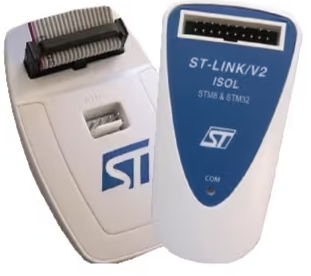
\includegraphics[width=0.5\textwidth]{figures/stlinkv2_original}
	\caption*{FONTE: ST-Microelectronics - ST-Link V2}
    \label{stlinkv2_original}
\end{figure}


\begin{figure}[ht]
	\centering
	\caption{St-Link V2 paralelo de fabricação desconhecida \cite{stlinkv2_cheap_ref}}
	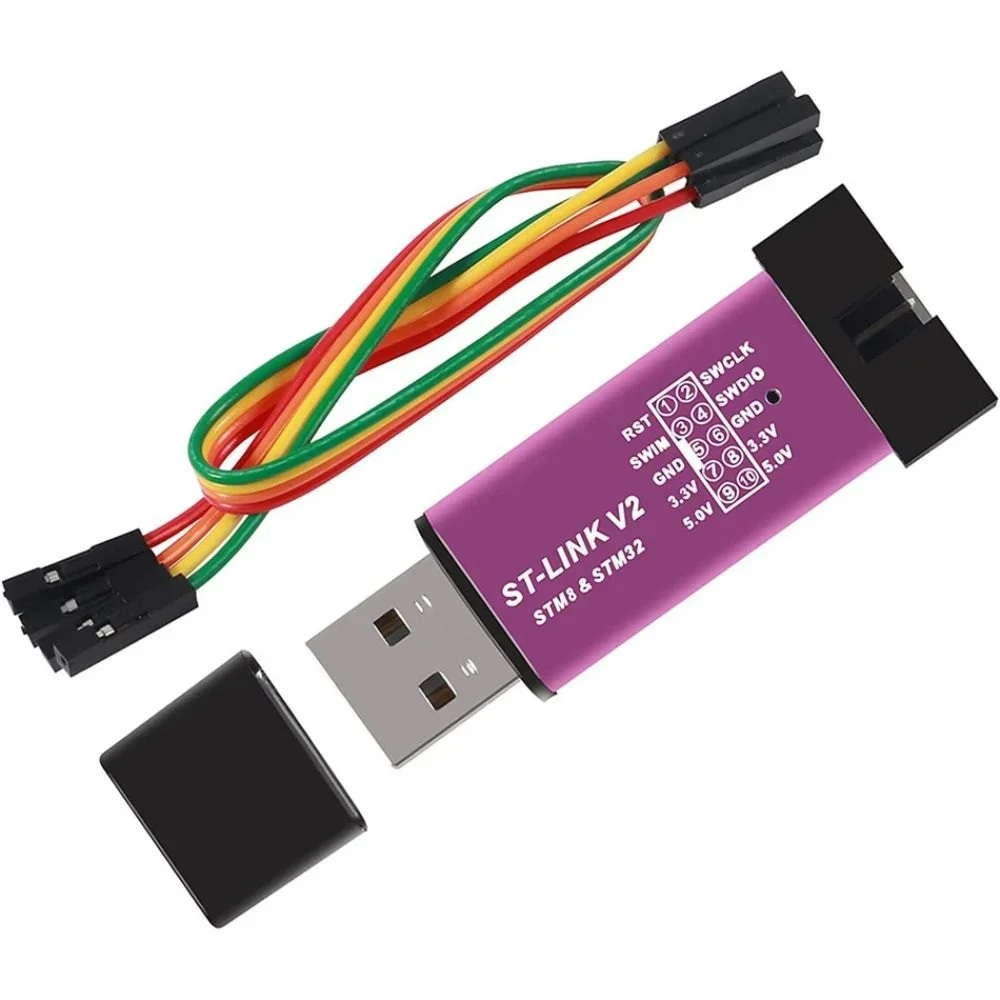
\includegraphics[width=0.5\textwidth]{figures/stlinkv2_cheap}
	\caption*{FONTE: https://www.achavevirou.com.br/gravador-st-link-v2-para-stm32-e-stm8}
    \label{stlinkv2_cheap}
\end{figure}


\begin{figure}[htb]
	\centering
	\caption{St-Link V2 paralelo e o problema da não padronização de pinos}
	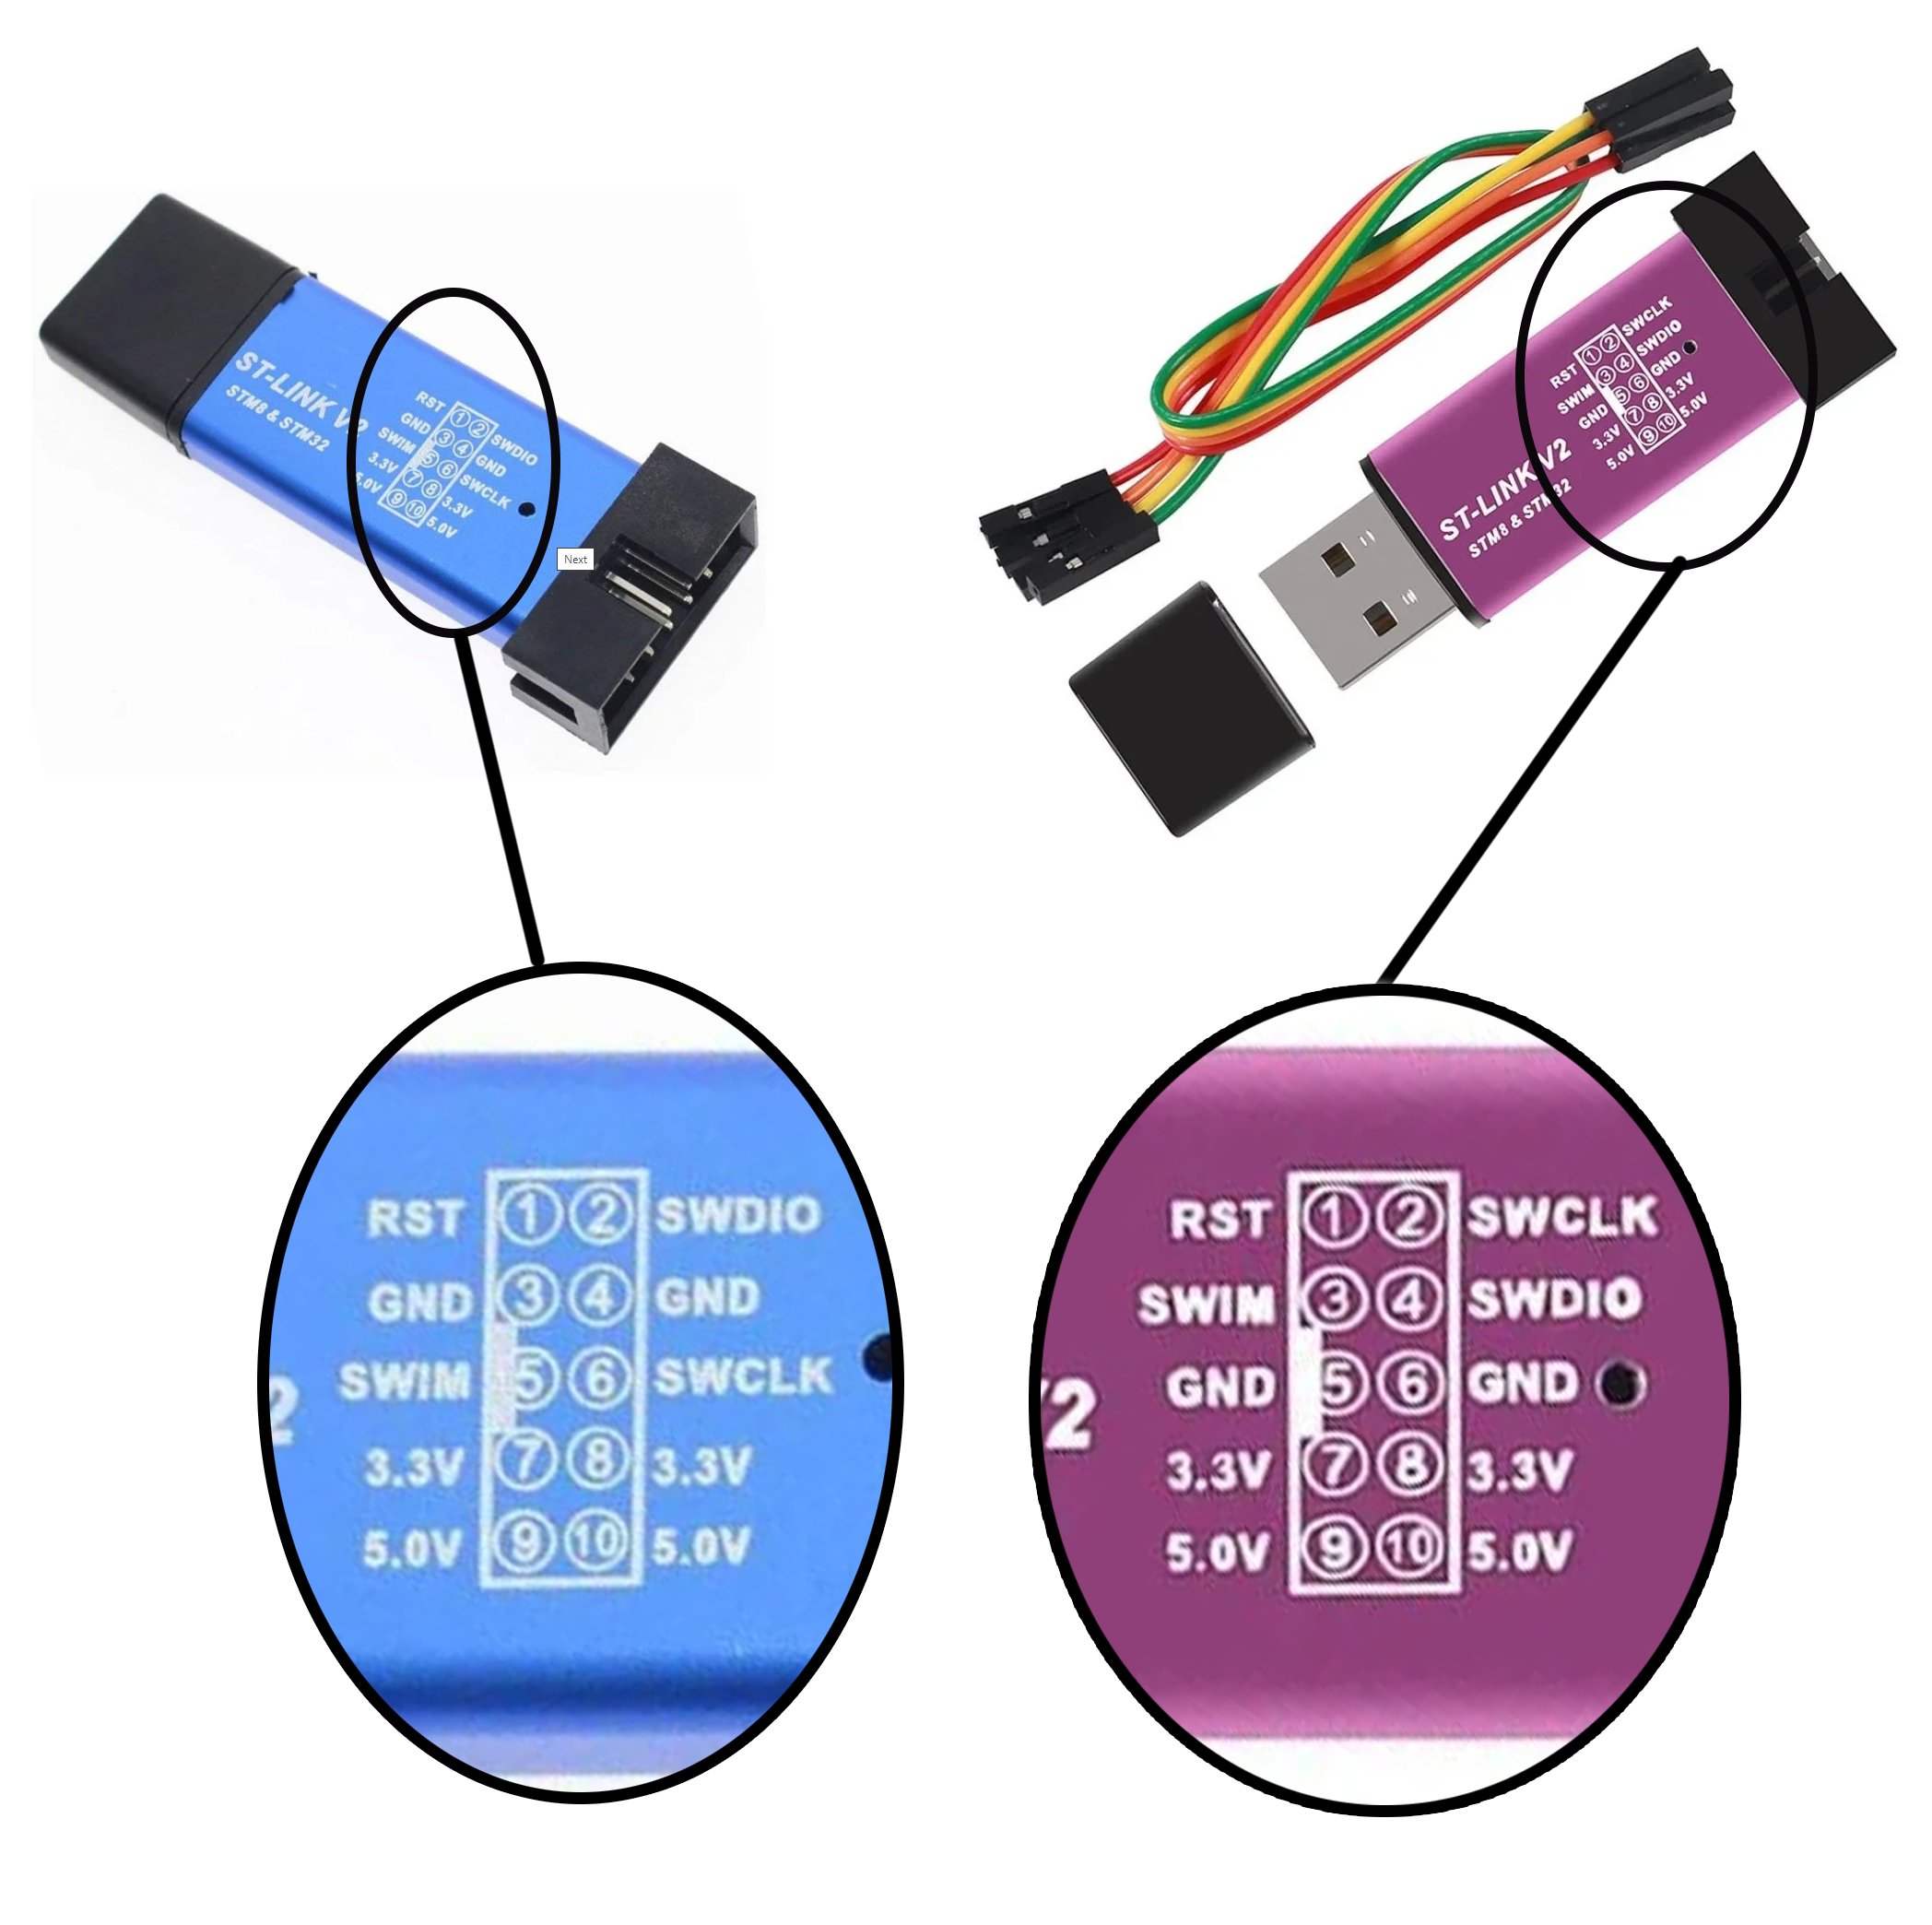
\includegraphics[width=0.5\textwidth]{figures/stlinkv2_cheap_pin_diff}
	\caption*{
		FONTE: Adaptado de https://universal-solder.ca/st-link-v2-usb-programmer-debugger/
		e https://www.achavevirou.com.br/gravador-st-link-v2-para-stm32-e-stm8
	}
    \label{stlinkv2_cheap_pin_diff}
\end{figure}

A partir desse ponto todas as menções a "STM32" são referem diretamente a  placa BluePill.


\subsubsection{ESP32 Devkit v1}

A placa ESP32 Devkit v1, de fabricação da DOIT.am, ela possui o microcontrolador ESP32-WROOM-32E (figura \ref{esp32_pinout}) fabricado pela Espressif Systems
A série ESP32 foi lançada em 2016 \cite{anuncio_esp32}, e possui arquitetura de 32 bits
tem se tornado popular por possuir opções com integração bluetooth e wifi.
O ESP32-WROOM-32E possui um processador dual core ESP32-D0WD-V3 \cite{esp32_wroom_32e_datasheet}, com frequência máxima de 240MHz, wi-fi 2.4Ghz de até 150Mbps e
bluetooth 4.2. Em relação aos periféricos, embora a placa tenha 48 GPIOs, elas estão endereçadas em apenas 25 pinos.
Entre os periféricos existem 15 canais ADC, 2 interfaces UART, 
2 canais DAC, 25 PWM, uma interfade de SPI, I2C e I2S, e 9 interface de toque capacitivo \cite{esp32_reference_2} \cite{esp32_reference}.

\begin{figure}[ht]
	\centering
	\caption{Diagrama de pinos do ESP32 Devkit v1}
	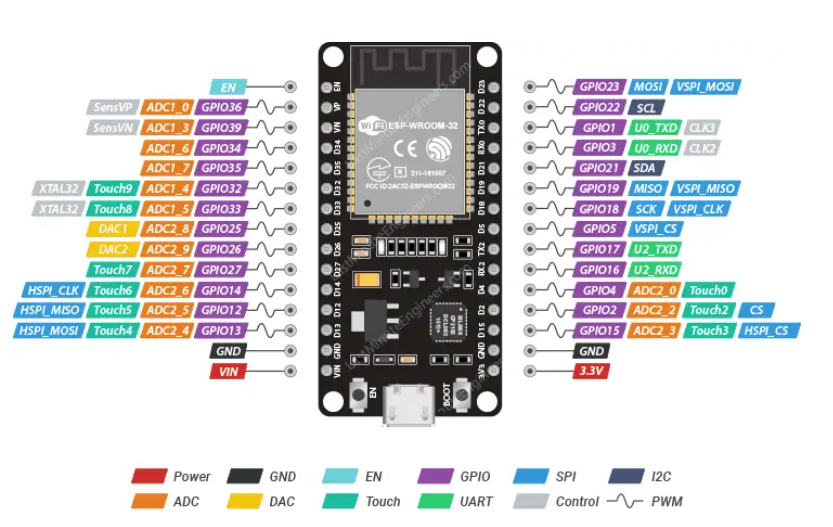
\includegraphics[width=1.0\textwidth]{figures/esp32_pinout}
	\caption*{FONTE: Adaptado https://lastminuteengineers.com/esp32-pinout-reference/}
	\label{esp32_pinout}
\end{figure}

De acordo com alguns artigos dispoíveis online sobre o ESP32 Devkit v1  \cite{esp32_reference_2} \cite{esp32_reference},
nem todos os 25 pinos são totalmente livres para usar,
alguns possuem limitações de uso de acordo como periférico em uso, a figura \ref{esp32_pinout_ref} resume as recomendações de uso do pinos.
Diferente do STM32 o ESP32 Devkit v1 pode ser gravado diretamente via USB.

\begin{figure}[ht]
	\centering
	\caption{Recomendação de uso dos pinos do ESP32 Devkit v1}
	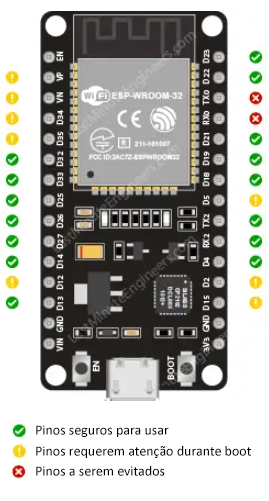
\includegraphics[width=0.35\textwidth]{figures/esp32_pinout_ref}
	\caption*{FONTE: Adaptado https://lastminuteengineers.com/esp32-pinout-reference/}
	\label{esp32_pinout_ref}
\end{figure}

A partir desse ponto todas as menções a "ESP32" são referem diretamente a placa ESP32 Devkit v1.


\subsection{IDE}

\subsubsection{Atollic TrueSTUDIO}

\begin{figure}[ht]
	\centering
	\caption{Interface Atollic}
	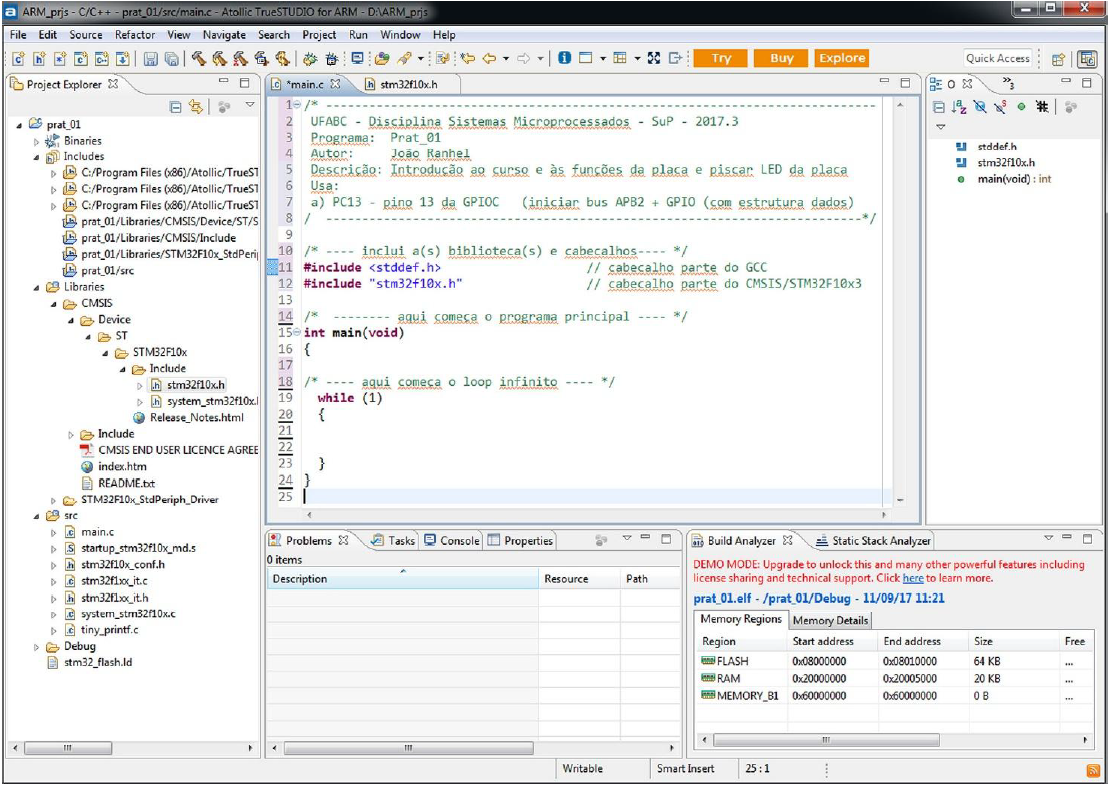
\includegraphics[width=0.8\textwidth]{figures/atollic}
	\caption*{FONTE: Sistemas Microprocessados -Apostila com práticas e foco nos processadores ARM CORTEX \cite{apostila_microprossados}}
\end{figure}

A IDE a ser usada para programar um STM32 seria o TrueSTUDIO, distribuído pela
Atollic, que foi adquirida pela ST-Microelectronics em 2017. Trata-se de um
software livre para programar em C/C++, criado com base na plataforma Eclipse,
e que possui todas as funções esperadas para o trabalho com o STM32, tais como
edição, compilação e debugging. Uma de seus principais vantagens é não haver
limites para tamanho de projeto, o que o torna ideal para trabalhos
profissionais. O TrueSTUDIO deixou de receber atualizações em 2017,
depois da aquisição pela ST-Microelectronics.\cite{apostila_microprossados}


\subsubsection{Arduino IDE}

Criado para ser a IDE das placa de desevolvimento Arduino, a primeira versão foi criada em 2005 \cite{arduino_id_history},
Mas as versões mais populares dispobilizadas ao público, são a 1.0.6 e 1.8. 
A versão 1.8 foi lançada em 2016 e recebeu atualizações até 2021, 
com a versão 2.0.0 lançada em 2022 \cite{arduino_tag_2}.

\begin{figure}[ht]
	\centering
	\caption{Interface Arduino}
	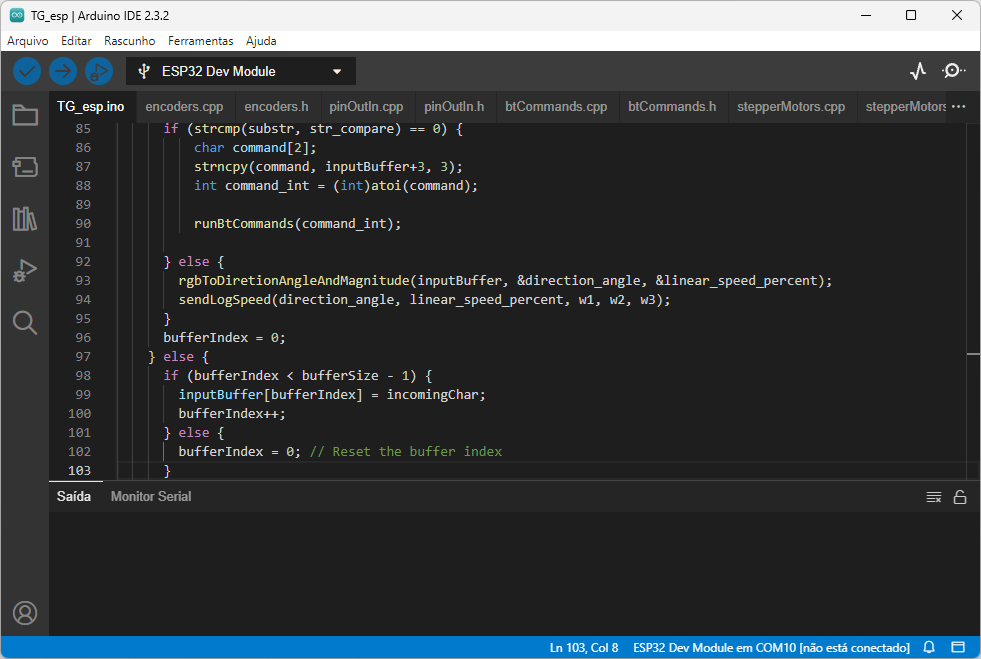
\includegraphics[width=0.9\textwidth]{figures/arduino}
	\caption*{FONTE: Própria}
\end{figure}

\subsection{Escolha do microcontrolador e IDE}

\subsubsection{IDE}

Devido a complicações nas configurações de múltiplas saídas de PWM com o
TrueSTUDIO, optou-se por usar Arduino como alternativa. Um obstáculo a essa
alternativa é que o Arduino não é compatível com STM32 nativamente,
porém o projeto Arduino\_STM32 \cite{arduino_stm32}, por Roger Clark.
O projeto contem os arquivos em C para usar o hardware do STM32 com Arduino IDE
do STM32 no Arduino. No momento de escrita deste trabalho, o projeto era
compatível apenas com a versão 1.8 da IDE do Arduino.

A escolha de usar a IDE do Arduino logo se tornou uma opção mais viável e flexível.
seja pela vasta lista  bibliotecas disponibilizadas por contribuidores e
documentações de projetos independentes. 

A IDE também é compatível com o ESP32,  usando a biblioteca arduino-esp32 \cite{arduino_esp32},
disponibilizada e mantida atualizada pela Espressif Systems.

\subsubsection{Microcontrolador}

Durante o desenvolvimento, o projeto foi migrado do STM32 para o ESP32 
devido a limitação do STM32 não poder ser conectado a porta serial via micro-USB-B e ST-link ao mesmo tempo,
e também de não poder deixar ligado o módulo HC-05 durante a gravação no STM32.
Sobre o módulo HC-05, em específico aos pinos de comunicação serial, se os pinos tiverem algum comportamento
diferente do padrão durante a gravação de um novo programa, esse comportamento pode danificar o módulo,
durante os teste, dois módulos foram danificados devido a excessivas vezes em que foram deixados
conectados ao STM32 durante a gravação de um novo programa.
E durante o uso STM32, algumas vezes a conexão via micro-USB-B permaneceu ligada ao mesmo tempo que o ST-link. 
A ocorrência excessiva dessa conexão levou a danificação do STM32.

Considerando esses pontos das diculdades encontradas com o uso do STM32, conexão via micro-USB-B e o módulo HC-05,
a placa ESP32 se tornou uma opção mais prática, pois já vinha integrado com bluetooth e podiaria ser conectado via micro-USB-B
para gravação e comunicação serial para debug ao mesmo tempo. E não seria necessário mudar de IDE e
seria necessário pouca alteração no projeto para adaptar o uso do bluetooth nativo.